\documentclass[twoside]{article}
\usepackage[a4paper]{geometry}
\geometry{verbose,tmargin=2.5cm,bmargin=2cm,lmargin=2cm,rmargin=2cm}
\usepackage{fancyhdr}
\pagestyle{fancy}


% nastavení pisma a~češtiny
\usepackage{lmodern}
\usepackage[T1]{fontenc}
\usepackage[utf8]{inputenc}
\usepackage[czech]{babel}

% odkazy
\usepackage{url}

\usepackage{float}
% vícesloupcové tabulky
\usepackage{multirow}
\usepackage{listings}
\usepackage{xcolor}
\usepackage{amssymb}
\usepackage{gensymb}
\usepackage{bbold}
\usepackage{amsmath}
\usepackage{siunitx}
\usepackage{mathtools}
\usepackage{commath}

% vnořené popisky obrázků
\usepackage{subcaption}

% automatická konverze EPS 
\usepackage{graphicx} 
\usepackage{epstopdf}
\epstopdfsetup{update}
%customize code listing
\definecolor{codegreen}{rgb}{0,0.6,0}
\definecolor{codegray}{rgb}{0.5,0.5,0.5}
\definecolor{codepurple}{rgb}{0.58,0,0.82}
\definecolor{backcolour}{rgb}{0.95,0.95,0.92}

\lstdefinestyle{mystyle}{
    backgroundcolor=\color{backcolour},   
    commentstyle=\color{codegreen},
    keywordstyle=\color{magenta},
    numberstyle=\tiny\color{codegray},
    stringstyle=\color{codepurple},
    basicstyle=\ttfamily\footnotesize,
    breakatwhitespace=false,         
    breaklines=true,                 
    captionpos=b,                    
    keepspaces=true,                 
    numbers=left,                    
    numbersep=5pt,                  
    showspaces=false,                
    showstringspaces=false,
    showtabs=false,                  
    tabsize=2
}

\lstset{style=mystyle}

% odkazy a záložky
\usepackage[unicode=true, bookmarks=true,bookmarksnumbered=true,
bookmarksopen=false, breaklinks=false,pdfborder={0 0 0},
pdfpagemode=UseNone,backref=false,colorlinks=true] {hyperref}

% Poznámky při překladu
\usepackage{xkeyval}	% Inline todonotes
\usepackage[textsize = footnotesize]{todonotes}
\presetkeys{todonotes}{inline}{}

% enumerate zacina s pismenem
\renewcommand{\theenumi}{\alph{enumi}}

% smaz aktualni page layout
\fancyhf{}
% zahlavi
\usepackage{titling}
\fancyhf[HC]{\thetitle}
\fancyhf[HLE,HRO]{\theauthor}
\fancyhf[HRE,HLO]{\today}
 %zapati
\fancyhf[FLE,FRO]{\thepage}

% údaje o autorovi
\title{KUI -- Výběr optimálního klasifikátoru}
\author{Vojtěch Michal}
\date{\today}

\begin{document}

\maketitle

\textit{Protokol o analýze a řešení úloh dle zadání na \cite{zadani}. Problem statement, jakož i značení a terminologie je vynecháno,
v případě potřeby ne nezbytné nahlédnout do zadání. Jména sekcí protokolu jsou ponechána dle zadání.}


\section{Výběr vhodného parametru}
V datech přiložených k zadání se nalézá tabulka výsledků klasifikátoru $C_1$ v závislosti na použité hodnotě parametru $\alpha$.
Protože je požadavek na \textit{vhodnost} stanoven velice obecně bez přiložení dalších testovacích dat, je nezbytné použít nějakou
metriku zohledňující pouze dostupné informace. Zásadní chybějící informací jsou vlastnosti \textit {ztrátové funkce}, která popisuje
mimo jiné závažnost chybných klasifikací -- False Positives (FP) a False Negatives (FN).

Bez znalosti ztrátové funkce není možné stanovovat rozumné požadavky na cistlivost a specificitu klasifikace, protože není zřejmé,
zda jsou například FN vůbec přípustné -- je snadné si představit autonomní auto, které se prostě stůj co stůj musí zastavit před člověkem,
i kdyby to znamenalo, že bude stavět u popelnic, značek, poštovních schránek a pouličních lamp. Nejrozumější metrika proto je nějaký poměr 
citlivosti jako funkce specificity parametrizovaný hodnotou $\alpha$, což je právě definice ROC křivky.

\begin{figure}[h]
	\centering
	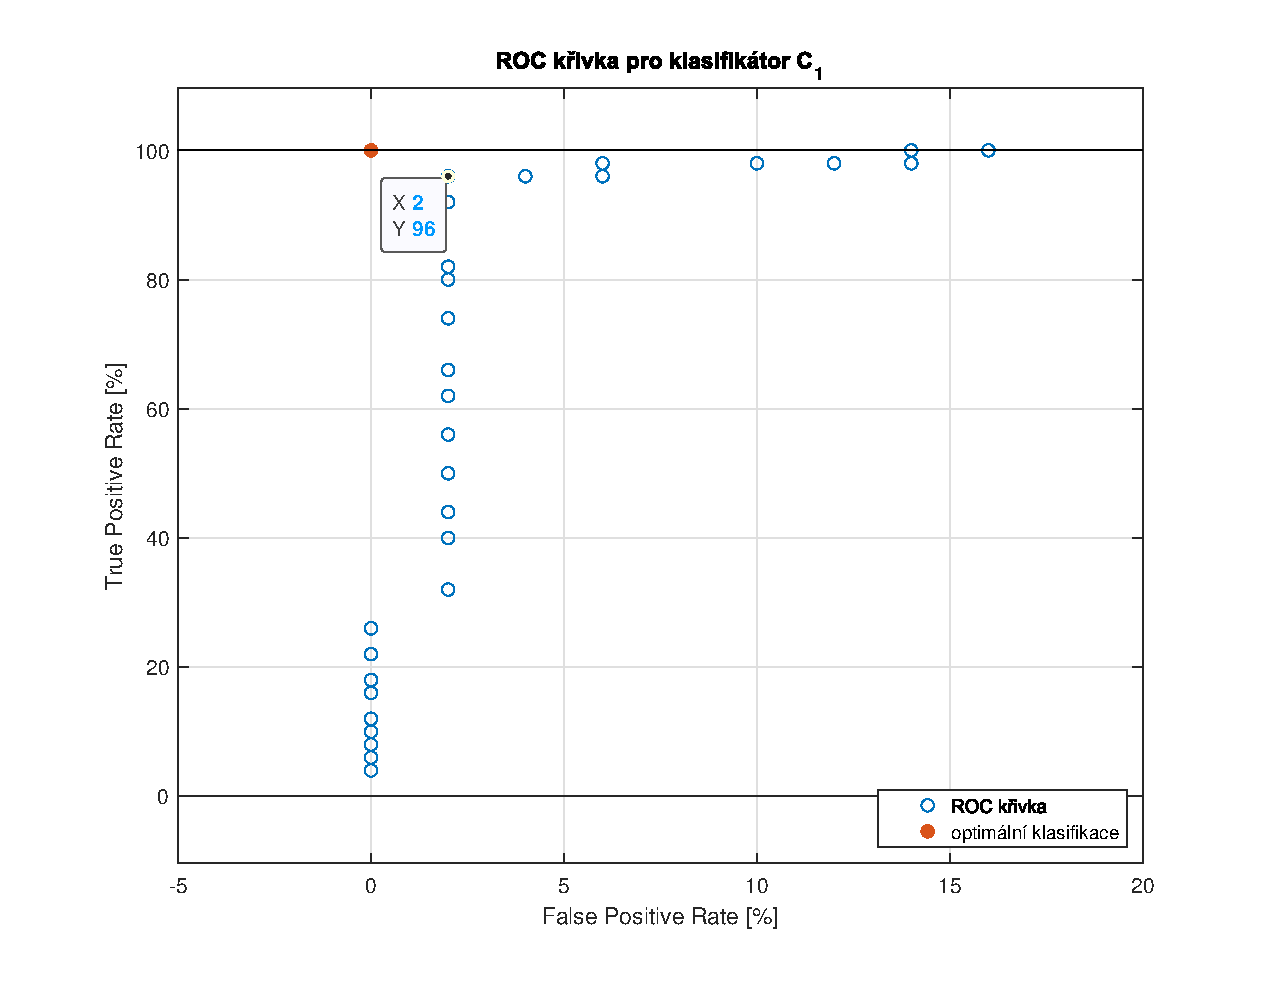
\includegraphics[width=0.6\textwidth]{roc.eps}
	\caption{ROC křivka pro $C_1$}
	\label{fig:roc}
\end{figure}

Pro klasifikátor $C_1$ je ROC křivka vykreslena na obrázku \ref{fig:roc}. Pro optimální klasifikaci je záhodno mít TPR~=~100 \%
a FPR = 0 \%, čemuž odpovídá červený bod v grafu. Nejblíže se mu nalézají parametry TPR~=~96 \% a FPR~=~2 \% dosažitelné pro
parametry $\alpha_{22, 23, 24}$.


\section{Přísně tajné!}
\label{sec:secret}
Zadání specifikuje ztrátovou funkci. Přeformuluji-li slova zadání do terminologie klasifikátorů, pak pro ověřování otisků prstů chci
\begin{enumerate}
	\item FPR~=~0 -- tedy stoprocentní specificitu -- abych měl jistotu, že otisk nikoho jiného nebude zaměněn za můj,
	\item TPR libovolný; když na to přijde tak klidně skoro nulový, protože mám nekonečně mnoho času na odemčení dat.
\end{enumerate}

Stěžejní požadavek na nulovou falešnou pozitivitu je splněn triviálně - prostě se data uzamknou a už nikdy k nim nikoho nepustíme.
V zájmu zdravého rozumu je ale záhodno nalézt dvojici (klasifikátor, $\alpha$), pro které bude požadavek na FPR~=~0 \% rovněž splněn,
ale doba odemykání bude rozumná (maximální TPR). Analýzou ROC křivek pro všechny klasifikátory $C_1$ až $C_5$ lze vyslovit závěr,
že klasifikátory $C_2$ a $C_3$ nejsou vhodné vůbec, protože nedousáhnou nikdy stoprocentní specificity. Ze zbylých klasifikátorů
se jako nejlepší kandidát nabízí dvojice ($C_4$, $\alpha_{11}$) s citlivostí 46 \% při zabráněnín všem falešně pozitivním výsledkům.

\section{Hlavně bezpečně}

S ohledem na výše dosažené výsledky lze predikát "býti lepším klasifikátorem" chápat jako požadavek na vyšší citlivost než 46 \%
dosažených v sekci \ref{sec:secret}. Na specificitě klasifikátoru již není nic co zlepšovat -- podařilo se dosáhnout stoprocentní
spolehlivosti, klasifikátor dávající jakýkoli horší výsledek je proto v zájmu bezpečí dat nepřípustný.
Pro posouzení nových algoritmů lze použít následující kód:


\begin{lstlisting}[language=Python]
	def classifier_is_permissible(reference, classification, required_FPR, minimal_sensitivity):
	# 'reference' is the correct classification. A list of 100 elements reference[sample]
	# 'classification' is the output to test. Format ... classification[alpha][sample]
	# 'required_FPR' and 'minimal_sensitivity' are the classifier parameters to beat
	num_alphas = len(classification) # the number of possible values of alpha
	scores = [] # stores (alpha, TPR, FPR) for each alpha
	for alpha in range(num_alphas):
		#get the total number of positives and negatives identified by the reference implementation
		P = sum(reference) # values are either 0 or 1
		N = len(reference) - P

		# Compute the number of correctly classified samples by the tested alhorithm
		TP = sum(x == 1 and x==y for x, y in zip(reference, classification[alpha]))
		TN = sum(x == 0 and x==y for x, y in zip(reference, classification[alpha]))
		FP = N - TN

		TPR = TP / P
		FPR = FP / N

	#extract only those values of alpha that achieve better results than our classification
	usable_alphas = [(alpha, TPR, FPR) for alpha, TPR, FPR in scores
	                    if FPR <= required_FPR  and TPR > minimal_sensitivity]

	if len(usable_alphas) == 0:
		return False # there is no parameter alpha for which the given classifier would be safer and faster

	# Extract the parameter with best score
	best_alpha, best_TPR, best_FPR = max(usable_alphas, key = lambda data: data[1])
	return True



#decide whether the new classifier is better:
our_TPR = 0.46
our_FPR = 0
is_better = classifier_is_permissible(ground_truth, new_classifier, 1, 0.46)
\end{lstlisting}


\begin{thebibliography}{9}

\bibitem{zadani}
	\emph{Zadání na stránkách KUI na CourseWare FEL ČVUT} \url{https://cw.fel.cvut.cz/wiki/courses/b3b33kui/cviceni/strojove_uceni/start}
\end{thebibliography}












\end{document}

